\defChapterTarget[ArchitecturalDesign]{Architectural design}
    \section{\textit{Overview}: High-level components and their interaction}
    The whole software that will become the main core of the SafeStreets
    initiative will be developed as a distributed application, which means that
    the software will be executed (or run) on multiple devices within a network.
    It will have a three-layers logic and be divided as following:
    \begin{itemize}
        \item \textbf{P}: The \textbf{\emph{presentation}} layer will handle all
        \textit{incoming} (\textit{and outcoming}) relations with the customers
        \item \textbf{A}: The \textbf{\emph{application}} layer will work as a
        "man in the middle" between the \textbf{P}resentation layer and the
        \textbf{D}atabase layer and will hold all the needed logic for the
        software to correctly work;
        \item \textbf{D}: The \textbf{\emph{database}} layer will be needed in
        order to store and manage all needed (and requested) information of the
        initiative;
    \end{itemize}
    Each and every one of the layers the architecture will be composed by a
    (group of) machines. By doing this, it is meant to provide, to each layer,
    its own dedicated hardware, for either scalability, failure handling and
    flexibility reasons.\\
    The following image shows the high-level architecture of the system without
    providing any detail of the components which will form the structure of the
    software itself, which will be tackled later in this document.
    \begin{figure}
        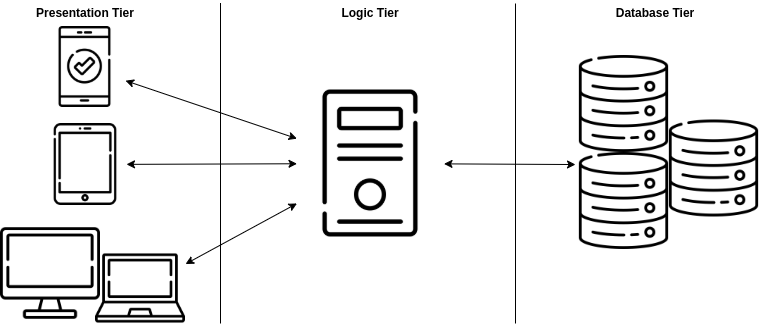
\includegraphics[scale=0.45]{dd/resources/images/HighLevelStructure.png}
        \caption{High-level architecture}        
    \end{figure}

    \section{Component view}
    \section{Deployment view}
    \section{Runtime view}
    \section{Component interfaces}
    \section{Selected architectural styles and patterns}    
        \subsection{Design Patterns}
            \subsubsection*{Model View Controller (MVC)}
    \section{Other design decisions}